\documentclass{article}
\usepackage{pgfplots}
\usepackage{filecontents}
\usepackage{tikz}
\usepackage{verbatim}
\pgfplotsset{compat=1.8}
\usepackage{pgfplotstable}
\newcommand{\scalefactor}{1}

\usepackage{graphicx}
\usepackage{caption}
\usepackage{subcaption}

\begin{document}

\begin{figure}
  \centering
  \begin{subfigure}[b]{0.3\textwidth}
    \centering
    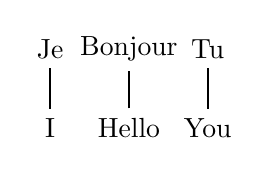
\begin{tikzpicture}
      \node at (0,0) (A) {I};
      \node at (0,1) (B) {Je};
      \node at (1,0) (C) {Hello};
      \node at (1,1) (D) {Bonjour};
      \node at (2,0) (E) {You};
      \node at (2,1) (F) {Tu};
      \draw[thick] (A) -- (B);
      \draw[thick] (C) -- (D);
      \draw[thick] (E) -- (F);
    \end{tikzpicture}
    \caption{A gull}
    \label{fig:gull}
  \end{subfigure}
  \begin{subfigure}[b]{0.3\textwidth}
    \centering
    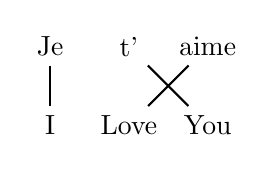
\begin{tikzpicture}
      \node at (0,0) (A) {I};
      \node at (1,0) (B) {Love};
      \node at (2,0) (C) {You};
      \node at (0,1) (D) {Je};
      \node at (1,1) (E) {t'};
      \node at (2,1) (F) {aime};
      \draw[thick] (A) -- (D);
      \draw[thick] (B) -- (F);
      \draw[thick] (C) -- (E);
    \end{tikzpicture}
    \caption{A tiger}
    \label{fig:tiger}
  \end{subfigure}

  \begin{subfigure}[b]{0.3\textwidth}
    \centering
    
\begin{tikzpicture}
      \node at (0,0) (A) {I Love You};
      \node at (0,1) (D) {Je t' aime};
    \end{tikzpicture}
    \caption{A mouse}
    \label{fig:mouse}
  \end{subfigure}
  \begin{subfigure}[b]{0.3\textwidth}
    \centering
    
\begin{tikzpicture}
      \node at (0,0) (A) {I Love You};
      \node at (0,1) (D) {Je t' aime};
    \end{tikzpicture}
    \caption{A mouse}
    \label{fig:mouse}
  \end{subfigure}
  \caption{Pictures of animals}\label{fig:animals}
\end{figure}




\end{document}
